\documentclass{article}
\usepackage{graphicx}

\setlength{\topmargin}{0in}
\setlength{\oddsidemargin}{0in}
\setlength{\textwidth}{6.5in}
\setlength{\textheight}{8.5in}

\newcommand{\vo}{\vec{v}_1}
\newcommand{\vt}{\vec{v}_t}
\newcommand{\xh}{\hat{x}}
\newcommand{\yh}{\hat{y}}
\newcommand{\be}{\begin{equation}}
\newcommand{\ee}{\end{equation}}

\begin{document}

\title{Two-dimensional Collision of Hard Balls}
\author{Drew Dolgert for Michael Fowler}
\date{\today}
\maketitle

We begin with two balls colliding, one moving, one at rest.
\begin{eqnarray}
\vo & = & v_1\hat{x} \\
\vec{v}_2 & = & 0
\end{eqnarray}
Immediately move to center of mass coordinates where
\begin{equation}
x_{\mbox{cm}}=\frac{m_1\vec{x}_1+m_2\vec{x}_2}{m_1+m_2}
\end{equation}
In these coordinates, the total linear momentum is zero.
\begin{eqnarray}
m_1\vec{v}_1+m_2\vec{v}_2 & = & 0 \\
m_1\vec{v}'_1+m_2\vec{v}'_2 & = & 0
\end{eqnarray}
The primes denote the velocities after the collision.
The effect of this momentum conservation on the kinetic energy
is that the particle velocities are related by
\begin{equation}
  \vec{v}_2 = -\frac{m_1}{m_2} \vec{v}_1,\qquad\mbox{and}\qquad
  \vec{v}_2'=-\frac{m_1}{m_2}\vec{v}_1'.
\end{equation}
Also, the speeds before and after the collision are unchanged
\begin{equation}
  v_1' = v_1,\qquad\mbox{and}\qquad v_2' = v_2.
\end{equation}
Because $\vec{v}_1$ and $\vec{v}_2$ are so well connected, we
can complete the calculation by studying $\vec{v}_1$ alone.

Our main physical consideration is the moment of impact of the
balls.  If we define an impact parameter, $B$, as the $\yh$
distance between the centers of the two balls, we can define
a single angle to describe the collision,
\begin{equation}
  \sin\theta = \frac{B}{2r}
\end{equation}
where $r$ is the ball radius.  For balls of differing radii, just use
$B/(r_1+r_2)$.  During a head-on collison, $\theta=0$.  A glancing blow
of $m_1$ above $m_2$ is at $\theta=\pi/2$ and below is at $\theta=-\pi/2$.
\begin{figure}
\centerline{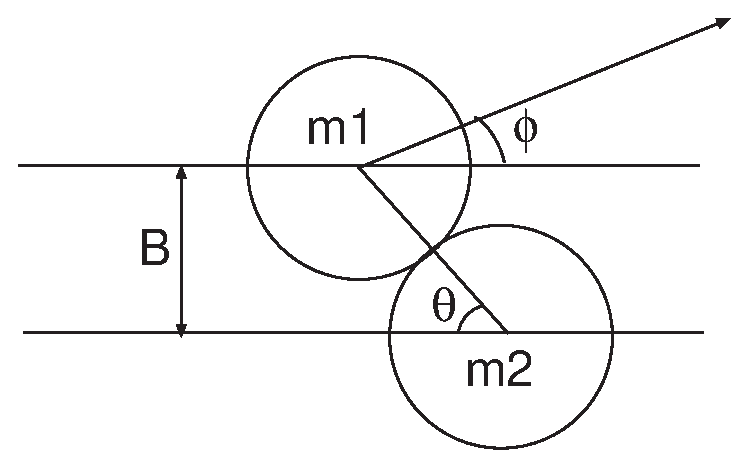
\includegraphics{angles.eps}}
\end{figure}


At the moment of impact, the impulse of the impact is along the point
of contact of the two balls.  For the first ball, we can write the impulse
as
\begin{equation}
  m_1(\vec{v}_1'-\vec{v}_1) = I (-\cos\theta\xh+\sin\theta\yh).
\end{equation}
The $\xh$ and $\yh$ components simplify to
\begin{eqnarray}
  m_1v_{1x}'-m_1v_1 & = & -I\cos\theta \\
  m_1v_{1y}' & = & I\sin\theta.
\end{eqnarray}
Making these a fraction gives us the needed angle,
\begin{equation}
  \tan\theta = \frac{m_1v_{1y}'}{m_1v_1-m_1v_{1x}'}=
  \frac{\sin{\phi}}{1-\cos{\phi}}.
\end{equation}
In the last step, we replaced $v_{1x}=v_1\cos{\phi}$ and
$v_{1y}=v_1\sin{\phi}$.  The angle at which $m_1$ leaves the collision is now
$\phi$ measured from the $\xh$ axis.
We now solve this equation.
\be
  \tan\theta-\cos\phi\tan\theta=\sin\phi
\ee
Squaring both sides gives
\be
  \tan^2\theta(\cos^2\phi-2\cos\phi+1)=\sin^2\phi=1-\cos^2\phi.
\ee
\be
  (\tan^2\theta+1)\cos^2\phi-2\tan^2\theta\cos\phi+\tan^2\theta-1 = 0
\ee
Using the quadratic formula, we find
\be
  \cos\phi=\frac{2\tan^2\theta\pm\sqrt{4\tan^4\theta-4(\tan^2\theta+1)
  (\tan^2\theta-1)}}{2(\tan^2\theta+1)}.
\ee
Simplifying shows
\be
  \cos\phi = \frac{\tan^2\theta\pm1}{\tan^2\theta+1}.
\ee
Clearly we take the negative root to find
\be
  \cos\phi = 2\sin^2\theta - 1 = 1-2\cos^2\theta.
\ee

With this simple solution, let's turn to technicalities.

\end{document}
